\documentclass[a4paper]{article}
\usepackage[english]{babel}
\usepackage[utf8]{inputenc}
\usepackage{amsmath}
\usepackage{amsfonts}
\usepackage{graphicx}
\usepackage{float}
\title{D \& D - Campaign: \\ Malidraxies}

\author{Adin Jasarevic}

\begin{document}


\begin{titlepage}
\maketitle
\end{titlepage}
\makeatletter
\renewcommand\thesection{}
\renewcommand\thesubsection{\@arabic\c@section.\@arabic\c@subsection}
\makeatother
\section{1: Introduction}
Malidraxies is a continent torn by chaos. The post-apocalyptic setting is a result of the war between the gods Vaxel god of corruption, and Vexil god of creation and rebirth. The aftermath of the war resulted in a magical fallout, and darkness has overtaken the world. The corruption slowly seeps across the planes and through the earth, only a few places are left unaffected by the disastrous transition. Most affiliated gods have been injured, some even left forgotten, and the world known to them has ended.\\ Subsequently the passage of time has left history soon to be buried, leaving only a glimpse of the past. With the world in ruins, civilisation has tried to adjust, but with the new world came the changes. Droughts, plagues and other disasters, were the least of people's worries, what came after was the most unnerving. In the beginning people thought nothing of it, but then it took a turn. It began as physical changes, one day you would wake up missing some teeth, or even discovering that your skin has lost all colour, but when madness spread, people were left horrified.\\
The surrounding continents of Phaalner, Grend, and Seramur have been trying to restrain the effects. Tirelessly searching for the cause of this catastrophe, while dooming the citizens of the once prospering continent to fend for themselves.\\
Society is now left intimidated and horrified by the prospect of adventuring and exploring. Only a few people are brave, or stupid enough to leave home following their intrepid dreams. But civilisation is in need of these morons. Not the treasures, stories, and achievements they leave home searching for, but the hope. Created by their sometimes shortsighted and rash decisions. Actions that could lead to a shift in this disaster that has left mankind baffled.
\newpage
\tableofcontents
\newpage

\section{2: History}
\subsection{Prehistory}
In the beginning all was void. But from rips in the fabric of nothingness radiance surfaced. The friction between these two powers created lacerations in space, and from these gashes the outer planes were created. These spiritual planes were the birthplaces of the first gods. It was here the first concepts of good, evil, chaotic and lawful were conceptualized.\\
These outer planes were chaotically swaying in the churning void, falling in and out of each others parallels, but as the inner planes conceptualized they worked as an anchor. Surrounded by the elemental chaos the material planes were created.\\
The gods sought power from this realm, and sometimes these interactions had unseen consequences. Other planes were created, some corresponding to the gods nature. The transitive and parallel planes such as the Ethereal plane, the Feywild, and the Shadowfell.\\
In an effort to stop the divide, the gods agreed to use mortals to settle their disputes and retreat to their own planes. The mortals who sought strength from the gods, became their messengers, and some were even awarded immortality or near godhood. Mortals who aided their deities could anticipate rewards such as "second lives". Mankind has since then been taken to the brink of destruction, and then reestablished many times. Many a time a god has strayed from their promise, interfering with the mortal plane, only time can tell what effect such occurrences will develop into.


\subsubsection{The Dragons}
There was an age a long time age, even before \textit{the great shift}, when dragons reigned over the material plane, at that time Tiamat lived in the Prime material plane, and was widely worshipped out of fear. Most creatures were left to live reclusive lives, and it was only after Pelor and Bahamut banished Tiamat to Tartarus, that true civilisation began to sprout.

\subsubsection{The Great Shift}
It is not known why but many fey species were seen populating the prime material plane in this era. From goblinoid infestations and lycanthropy to elves and gnomes, many creatures and diseases began migrating to Nixera. 



\subsection{The Sibling Strife}
Not much is known about the war. Only the effects of the drawn-out battle are clear. 
 
\subsubsection{Instigation}
Most say the war was a result of a long drawn out plan Vaxel concocted in order to cage Vexil in the prime material plane, ending the powerstruggle between the siblings.

\section{3: The world}
Nixera is a large world with 5 continents
\subsection{Phaalner}
Is called the endless continent. No one knows how much is left unexplored and many believe this land is endless. There is a river that splits 

\subsubsection{Halfling society}
Halflings are usually simple creatures, they fit into every civilization, and usually live simple lives. They are usually a happy people, some wander, others stay in their burrow cities for their whole lives. 

\subsubsection{Æmilie's burrow city}

\subsubsection{Hazeltown}
A large independent city, with a large cultural history. The biggest attraction of this city is their winters crest festival, a festival that commemorates the new year, the middle of winter, and the solstice. It is viewed as a turn for the better, and a brief cross of the planes.

\subsubsection{Ferrildal}
A large imperial capital of the Yu empire. Emperor Yu, an old existence is the king of this large empire, that mainly reins over the eastern side of the \textit{Shijebi river}. It is made of four districts. The goldenblue district, with plenty of space for the large merchant companies living quarters, and storehouses. The sapphire district is where most envoys, ministers, and other highborn folk live, most buildings go from exquisite blue to cyan and purple. The cyan district, where the most of the city's population is cooped up in narrow streets, where some places even have more layers, \textit{here lies a crime syndicate}. The marked district, is the central district where the learned folk do their business. Even more than a place of exchange, this district seems like a large stage, where most handiwork is done with large audiences.

\subsubsection{The Sandless Desert}
40 km outside of Ferrildal lies a vast desert of sandstones, where jagged cliffs reach the skies.


\subsubsection{Shijebi river}
Some say that the gates to Tartarus are at the end of the river, and that the titans of old are kept back by the rivers tide.

\subsubsection{Jade Citadel}
Gigantic fort-like structure, lots of protective orbs of differing colors holding spells.

\subsection{Grend}
is the largest and most eastern continent. Most of the continent is controlled by different human kingdoms with varying degrees of independence and isolation.

\subsubsection{Draconia}
Draconia is the kingdom of the dragonborn. Their society is extremely isolated from other societies, and therefore also very unique. Most dragonborns seek power, and their hierarchy is build for the acquisition of power. There are very strict rules forbidding especially killing dragonborn with the exception of revanants because they are lower beings.
\\
\textbf{Clan structure}
Some dragonborn thought collaboration would give them a chance to acquire the power they seek, so some banded together which at some point created the clans.
\\
There are seven major clans consisting of Tyraqis (mostly red) Darghus (mostly white) Varhdrhe (only green and black) Shrrewh (mostly blue) Gruuh (black, white, and red) Drackt (mostly green and blue), and Phreesh (mostly black)
\\
\textbf{Tyraqis}
The Tyraqis clan consists of red dragonborn, with slight color variations like orange dark, light or  near yellow scales. Their clan is very arrogant, and believes itself to be the strongest clan. The internal hierarchy is dependent on strength, they have a board of the five strongest members of their clan, and a chief which makes decisions for the clan. The boards decisions are law, and if you don't follow the orders of those stronger than you, battle can decide the dispute.
\\
\textbf{Power struggle}
The power struggle mostly happens behind the scene. There are countless rivalries between dragonborn, and a part of them thinks it is fun to play this type of political game. 
\\
\textbf{The military}
The hierarchy in the military is much like their clans dependent on strength, both physical and influential. The main army of draconia is very large, but they also have a division of wyvern-riders called the sunwing, who are proven warriors that combat most of the dangers found in their mountain range.

\subsubsection{Temple of the immortal}
The Immortal cultivators were a people that tried to transcend the physical body, reaching for superhuman abilities. Most of the people in the temple consisted of trainees, or teachers too old to travel or break through the threshold to immortality.
\\
The highest position in the order was that of the sky-hierarch, the leader of their people.
\\
\textbf{Transcending the mortal body}
Transcendence could either be achieved through travel, or cultivation in the transcendence-hall. This construct was made not too long ago, but was a rift in space which channelled a miasma, the teachers called the immortal mist.
\\ Training in the hall was dangerous, therefore it demanded constant vigilance over soul and body.
\\ It was not everyone that was gifted to the extend of reaching immortality, first one had to build up their body so that they could resist the effects of the godmist while gaining the benefits.
\\
\textbf{Sacred ground}
The temple had often been called a sacred ground because of their reputation of protection against forces that threatened the prime material plane. It was even said that many great evil artefacts had been sealed inside the temple.

\textbf{Destruction}
After an incident that happened just around the time that a new batch of disciples would be introduced into the path to immortal cultivation, most cultivators of the immortal way disappeared.




\subsubsection{Deep gnome society}
In dark caverns deep under the earth a society of deep gnomes prosper in Grent. Since the illithid civilisation was ruined, and their terror-regime ended, a large population of deep gnomes have banded together and formed the city Darkcave. The name Darkcave was decided by the founders of their civilisation who thought this name was extremely descriptive and therefore would keep any misunderstandings from happening when they chose to try connecting to the outside world.
\\
\textbf{Dark library}
The Dark library is the deep gnomes only reliable way of attaining knowledge of the outside world, and you could say becoming a librarian there is the most prestigious post a gnome could have in their society. Knowledge demands respect and this is especially true when the recipients of that knowledge know nothing. As a librarian you are chosen from young because of your aptitude for learning and teaching. All Dark librarians are wizards or priests, and their quest is to acquire as much information about the outside world, help in diplomatic missions, and help giving deepgnome society a voice in the outside world. Every fifty years a bunch of gnomes are send to the outside world to increase their skills and thereby setting their status in Darkcave.
\\
\textbf{High Dark Librarian} 
The High dark librarian is the most important position in the library, without him the Darkcave civilisation would perish. The only way to become a High Dark Librarian is by travelling to the five continents and gaining access to the five great libraries. This journey requires wit, power, and most importantly leadership. This is often done by becoming a leader of a group, thereby learning the skills necessary to lead the people and proving their aptitude for magic and knowledge. A new high librarian hasn't been chosen for the last 300 years, and without the knowledge gained from all five libraries the Darkcave people are frightened by the possibility that their ties with the outside world will be broken.
\\

\subsubsection{Saghoon}
Saghoon is a large harbour city. This city has the sky-district where the king's palace, and other major power's houses are placed. Here the king reins over his territory.
\\
\textbf{The Adamantium Stash}
The Adamantium Stash is the largest library in the continent, containing valuable information gathered throughout the ages. It has a close relationship with the other four libraries, and a secret relationship with the plane of arcadia. The priests that are seen walking in and out of the library are acolytes seeking knowledge in order to impress their chosen gods. This knowledge is gained by copying the books they are each given to study, so that the library can gain an ever expanding collection. Other than that they are hired to make sure that no books are neglected and thereby damaged.   

\textbf{The brief lady}
The brief lady is a tavern establishment between the docks and the marked of the city on the other side of the sky-district.

\subsection{Seramur}
In elfish Seramur means land of the west, or land of desert-winds. Large parts of this continent are arid.

\subsubsection{Goliath society}
In the mountainous region in southern Seramur two tribes of goliaths roam they have minor grievances, and most disputes stem from their competitive spirit. One tribe consisting of 37 goliaths is lead by the Stormborn, the other 57 goliaths strong is lead by Durock Brassjaw.
\\
\textbf{Appeasing the mountain}
Most goliaths fear the mountain of Onyxis, not for fear of burning or dying, but for fear of other's misfortune. Centuries ago the goliaths angered the mountain, after many days of black sky a thunderous voice rang, and demanded the tribes gave it gifts of gold and meat, stating otherwise it would burn the world. The skywatchers of both tribes decided to give this task to one goliath that would collect the gifts of both tribes and present them to the mountain. This position was called Firekeeper, and every 3 years the Firekeeper would have to travel up the mountain to deliver the treasure while also communicating with the fire. Even though the job of a Firekeeper was important. It also demanded near constant vigilance over the flame-mountain, which resulted in most Firekeepers becoming distant from their tribes. 
\\
\textbf{Onyxis}
In the depths of the mountain lies a creature that can rival deities. The phoenix Onyxis, is in the middle of his reincarnation cycle, and now that he has reformed a fragment of his former power he has coaxed a goliath into following him to further his reach into the prime material plane. But to do this he needs to be set free of the power that binds him to the fire-elemental plane. Onyxis is called the all-destroyer, Cleanser of worlds, the ever burning flame and the mad burn. Even as an chaotic evil god he harbours hatred towards the corrupting miasma in Malidraxies, because only in the mountains of dramour will he be able to cross to the prime material plane. His whole purpose is to set the world aflame in order to see a knew one appear from the ashes, only in this way can the world become stronger like most metals the impurities that inhabits the world can only be removed by reforging it.


\subsubsection{Ralehh}
Elven city with harbour in the bottom part of Seramur. There is a large part of the society that is poor, and have need for food, because the arid climate makes harvests poor. They get by, by using magically grown fruits and vegetables.

\subsection{Seramir}
In elvish Seramir means land of the east, or land of frozen heart. As supposed to the real world, because of Nixera's two suns there is only one cold pole on this plane.

\subsection{Malidraxies}

\subsubsection{Dwarven settlement of Dragon's reef}
A large hole, that gets gradually deeper. Now nests of wyverns, and other beasts inhabit the former dwarven settlement. There is also a large population of Duergar that have made this place their home.

\subsubsection{Mordred the Cogcity}

\subsection{Sambalba}
Small foggy swamp city, with a makeshift dock. old houses where some have sunk into the landscape. large roads going from the city making  

\subsection{Characters}

\subsubsection{Lijiang}
A samurai from the western part of Phaalner very competitive and speaks in third person. Has fought people from all over the world.

\subsubsection{Ava}
a black draconian knight. Big and strong 9th level warrior, trained wolff's character, and always up for a challenge.

\subsubsection{Jharkhand}
A gnome druid with an extremely fast breed of dog. with his magic he has enhanced his dog.

\subsubsection{Fenris}
Fenris and his old master Agotash were the Greywardens. Greywardens were tasked with protecting the world against the threat of chromatic dragons, at a time when they prospered. This was at a time when Tiamat lived in the prime material plane, and Fenris' master Agotash a powerful stone giant, helped banishing Tiamat, alongside a few heroic characters that reigned supreme at the time, and Bahamut and Pelor into Tartarus. Before this long drawn-out battle Agotash sealed Fenris away in a locket at a temple in the mountains of Phaalner. Fenris knew this age as the Age of Arcanum an age within the Dragonage, where magic was experimented with to find a way to stop the dragon-plague, but this was so long ago that the world has mostly forgotten the time. At this time the Behir was carved by giants in order to combat dragons.

\section{4: The Astral sea}
\begin{figure}[h]
\begin{center}
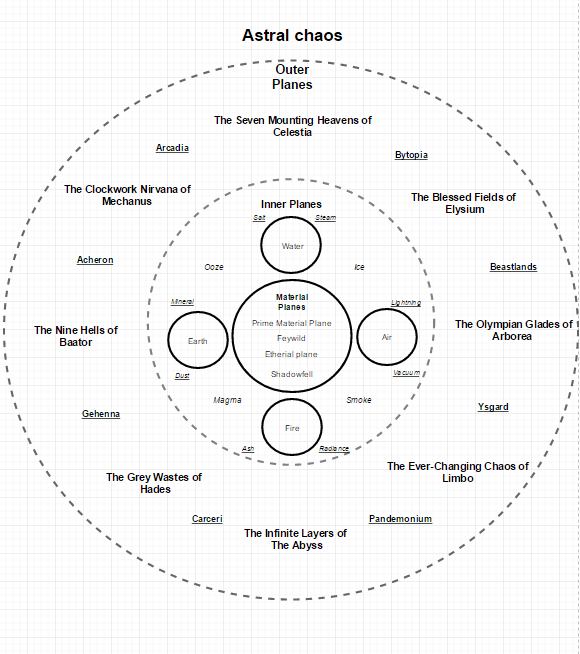
\includegraphics[scale=0.8]{TheAstralSea}
\caption{Depiction of the Astral sea, in the Great wheel model.}\label{TheAstralSea}
\end{center}
\end{figure}

\subsection{The feywild}

\subsubsection{Yuankhan - The ape king}
An archfey cursed with lycanthropy. Yuankhan is of elven heritage from before most journeyed to the prime material plane. He was cursed by a chaotic good god (or godlike) creature living in the Beastlands to live the rest of his life as a wereape because of his show of disgust towards that gods daughter. In his half-crazed and embarrassed state he retreated to his home sending it to the sky, where he planned to spend the rest of his life brooding. 

\textbf{The cloud temple of Baimenhu}
Baimenhu now lays half destroyed after many years of neglect in most of the island has broken off. In the portal-room there are 4 portals powered by a crystal which also gives them a shared "ID". Right now the powered portal is the portal to the prime material plane near the small village of Hazeltown in Phaalner. Other than that a portal to the lower reaches of the Feywild, a portal to the Beastlands, and a portal to the Wind elemental plane remain.

\begin{figure}[h]
\begin{center}
\includegraphics[scale=0.15]{Baimenhu1st}
\caption{A map of the remaining first floor of Baimenhu.}\label{Baimenhu1st}
\end{center}
\end{figure}

\begin{figure}[h]
\begin{center}
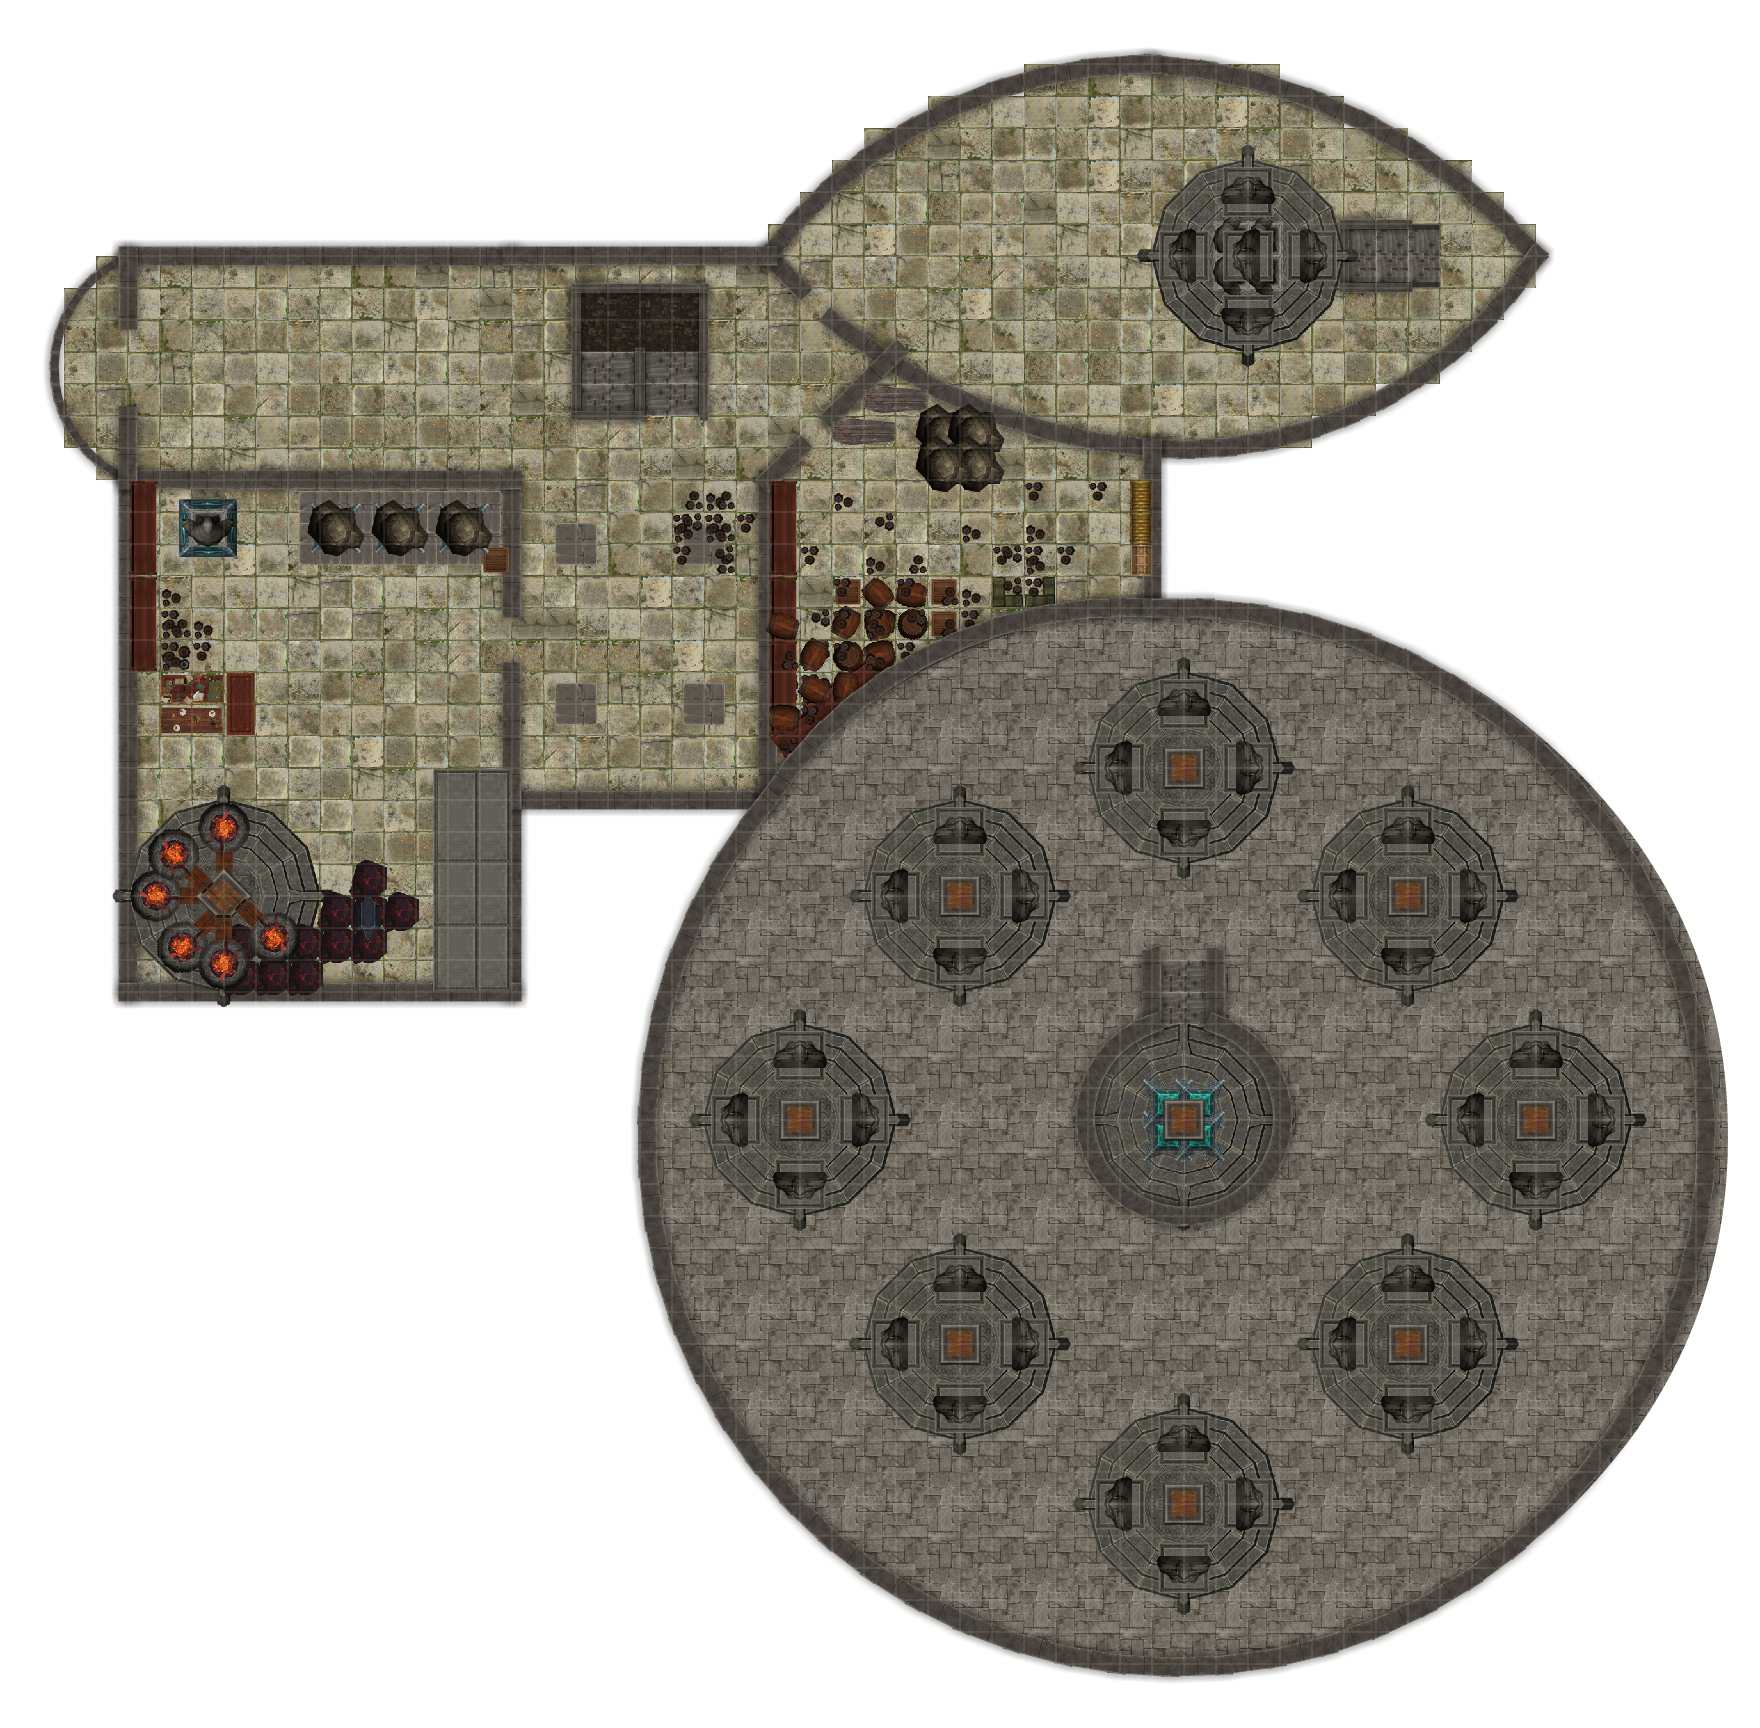
\includegraphics[scale=0.2]{Baimenhu2nd}
\caption{A map of the remaining second floor of Baimenhu.}\label{Baimenhu2nd}
\end{center}
\end{figure}
\section{5: Character races}

\section{6: Character classes}

\section{7: Mutations}

\section{8: Magic}

\section{9: Equipment}

\section{10: Magic items}

\section{11: Monsters}

\section{12: Pantheon}

\subsection{Vaxel}
Vaxel, also known as \textit{The Silent Menace}, \textit{The Coming Madness}, and \textit{The Overseer of Change}, is a chaotic evil intermediate deity of Corruption, Change and Madness. Vaxel's acolytes believe that through giving their mind and reason over to Vaxel, they can gain the power to change. Vaxel's symbol is a rotten brain.\\


\subsection{Vexil}
Vexil, also known as \textit{The Restoring Mistress}, \textbf{The Rebirth Catalyst}, and \textbf{The White Mistress} is a neutral good intermediate deity of creation, renewal, and peace. Vexil's priests believe that one shouldn't change themselves to overcome their faults, but that true peace is found when one accepts who they are. She values wisdom over all else, and her symbol is a standing person.

\subsection{Ghourr}
The second sun


\end{document}